\thispagestyle{hoccungpinone}
\pagestyle{hoccungpi}
\everymath{\color{hoccungpi}}
\graphicspath{{../hoccungpi/pic/}}
\blfootnote{$^{1}$\color[named]{hoccungpi}Giáo viên trường THPT Chuyên Trần Phú, Hải Phòng.}
\begingroup
\AddToShipoutPicture*{\put(0,616){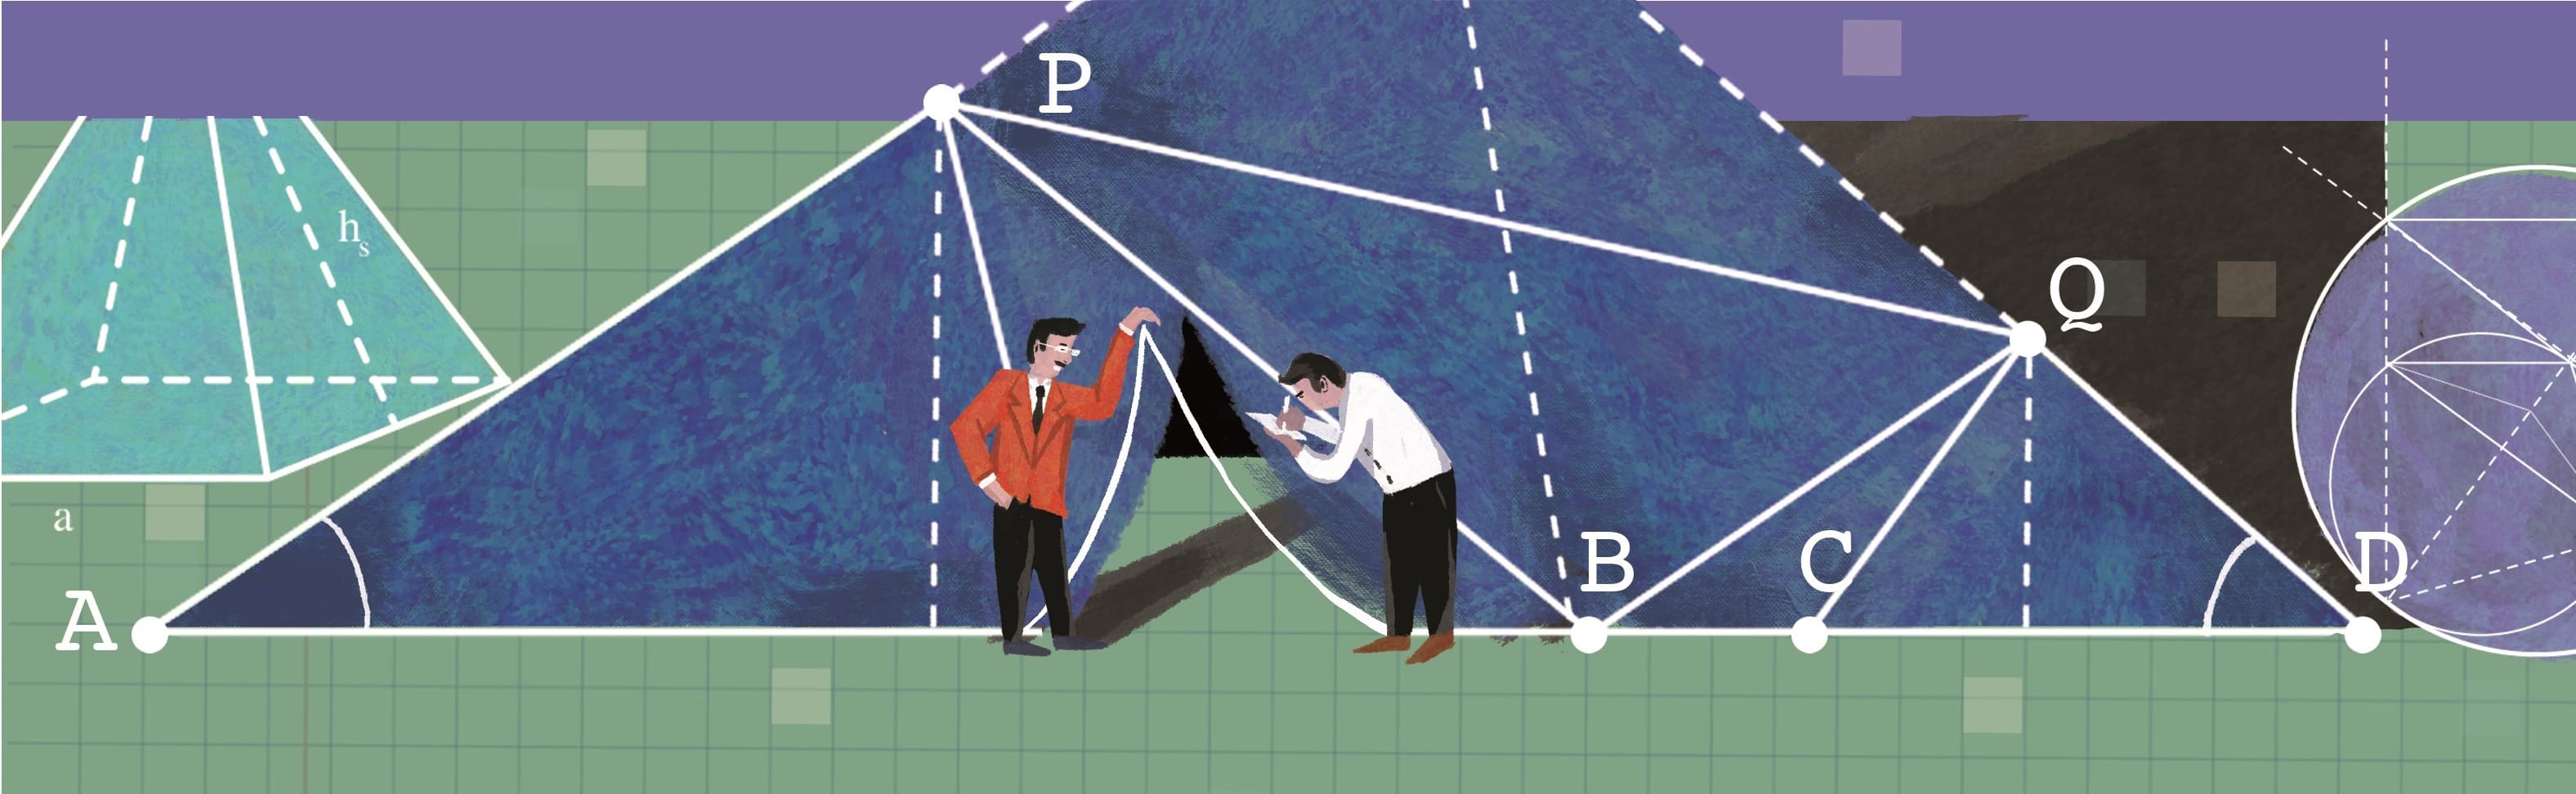
\includegraphics[width=19.3cm]{../bannerhoccungpi}}}
\AddToShipoutPicture*{\put(65,495){
\includegraphics[scale=1]{../tieude.pdf}}}
\centering
\endgroup
\vspace*{215pt}

\begin{multicols}{2}
	\textbf{\color{hoccungpi}A. Giới thiệu}
	\vskip 0.1cm
	Trong đề thi chọn học sinh giỏi quốc gia năm $2022$ có bài toán phương trình hàm sau:
	\vskip 0.1cm
	\textbf{\color{hoccungpi}Bài toán $\pmb{1.}$ (HSG Quốc gia $\pmb{2022}$).}
	Tìm tất cả các hàm số $f:\mathbb{R^+}  \rightarrow\mathbb{R^+} $ thoả mãn
	\begin{align*}
		f\left(\frac{f(x)}{x}+y\right)=1+f(y)
	\end{align*}
	với mọi số thực dương $x$, $y$.
	\vskip 0.1cm
	Bài viết này, chúng tôi xin được trình bày lời giải cho bài toán $1$ (mục $B$); sau đó là trình bày bài toán tổng quát (bài toán $2$), mà bài toán $1$ chỉ là một trường hợp riêng của nó (mục $C$). Mục cuối cùng (mục $D$) là ứng dụng của bài toán tổng quát để giải một số bài toán phương trình hàm đi từ $\mathbb R^+$ vào $\mathbb R^+$. 
	Mặc dù bài toán $2$ có ứng dụng rất mạnh mẽ và bất ngờ, tuy nhiên vẫn có một vài bài toán thỏa mãn các giả thiết của bài toán $2$, nhưng khi ta áp dụng bài toán  $2$ thì vẫn không thu được kết quả nào đáng kể. Bài viết này cũng sẽ giới thiệu một vài bài toán như thế để các em học sinh giỏi và các thầy cô giáo tham khảo.
	\vskip 0.1cm
	\textbf{\color{hoccungpi}B. Lời giải bài toán $\pmb{1}$}
	\vskip 0.1cm
	Giả sử tồn tại hàm số 
	$f:\mathbb{R^+}  \rightarrow\mathbb{R^+} $ thoả mãn
	\vskip 0.1cm
	\hspace*{40pt}$f\left(\dfrac{f(x)}{x}+y\right)=1+f(y)$ \hfill ($1$)
	\vskip 0.1cm
	với mọi số thực dương $x$, $y$.
	Từ ($1$) ta có
	\begin{align*}
		&f\left( {\frac{{f(x)}}{x} + y} \right)=1+f(y),\\
		&f\left( {\frac{{f(z)}}{z} + y} \right)=1+f(y).
	\end{align*}Do đó 
	\begin{align*}
		f\left( {\frac{{f(x)}}{x} + y} \right) = f\left( {\frac{{f(z)}}{z} + y} \right)\tag{$2$}
	\end{align*}
	với mọi số thực dương $x$, $y$, $z$.
	\vskip 0.1cm
	$1)$ Giả sử $f$ là đơn ánh.
		Từ ($2$) ta suy ra
		$\dfrac{{f(x)}}{x} = \dfrac{{f(z)}}{z}$ với mọi số thực dương $x$, $z$.\\
		Do đó $f(x) = cx$ với mọi số thực dương $x$ (với $c=f(1)$); thay vào ($1$) ta được
		$c=1$. Vậy
		$f(x) = x$ với mọi số thực dương $x$.
		\vskip 0.1cm
	$2)$ Giả sử $f$ không là đơn ánh.
		Khi đó tồn tại các số thực dương $a<b$ sao cho $f(a)=f(b)$.
		Từ ($2$) ta có
		\begin{align*}
			f\left( {\frac{{f(a)}}{a} + y} \right) = f\left( {\frac{{f(b)}}{b} + y} \right)
		\end{align*}
		với mọi số thực dương $y$. 
		Từ đây, thay $y$ bởi $x - \dfrac{{f(b)}}{b}$,
		ta được
		\begin{align*}
			f(x + T) = f(x)
		\end{align*}
		với mọi số thực $ x > \dfrac{{f(b)}}{b}$,
		(với $T = \dfrac{{f(a)}}{a} - \dfrac{{f(b)}}{b} > 0$).
		Bằng quy nạp, ta được
		\begin{align*}
			f(x) = f(x + nT)
		\end{align*}
		với mọi số thực $x > \dfrac{{f(b)}}{b}$ và số nguyên dương
		$n$.
		Từ ($1$), cho $x=1$, ta được 
		\begin{align*}
			f\left( {y + \alpha } \right) = f(y) + 1
		\end{align*}
		với mọi số thực dương $y$ (với  $\alpha  = f(1)$). Do đó
		$f\left( {y + n\alpha } \right) = f(y) + n$
		với mọi số thực dương $y$ và số nguyên dương $ n$.
		Xét một số thực  $x > \dfrac{{f(b)}}{b}$ bất kỳ. Chọn số nguyên dương $n>f(x)$,  rồi chọn số nguyên dương $k$ sao cho $kT > n\alpha $, khi đó
		\begin{align*}
			f(x)&= f(x + kT) = f\left( {x + kT - n\alpha  + n\alpha } \right)\\
			&= f\left( {x + kT - n\alpha } \right) + n > n > f(x);
		\end{align*}
		ta gặp mâu thuẫn. 
	\vskip 0.1cm
	Vậy, có duy nhất hàm số thỏa mãn yêu cầu đề bài là
	$f(x) = x$ với mọi số thực dương $x$.
	\vskip 0.1cm
	\textbf{\color{hoccungpi}C. Bài toán tổng quát}
	\vskip 0.1cm
	Bài toán $1$ chỉ là một trường hợp riêng của bài toán 
	$2$ sau đây.
	\vskip 0.1cm
	\textbf{\color{hoccungpi}Bài toán} $\pmb{2.}$
		Cho các hàm số $f, g, h: \mathbb{R}^{+} \rightarrow \mathbb{R}^{+}$ thỏa mãn
		\begin{align*}
			f(g(x)+y)=h(x)+f(y)
		\end{align*} 
		với mọi số thực dương $x, y$. Chứng minh rằng  $\dfrac{g(x)}{h(x)}$ là hàm hằng.
		\vskip 0.1cm
		Bài toán $2$ này có ý nghĩa quan trọng, nó cung cấp thêm cho chúng ta một công cụ hữu hiệu để giải một số bài toán phương trình hàm đi từ 
		$\mathbb{R}^{+}$ vào $\mathbb{R}^{+}$. 
		\vskip 0.1cm
		\textit{Lời giải.}
			Ký hiệu $P(x, y)$ là mệnh đề $f(g(x)+y)=h(x)+f(y)$, với $ x$, $y$ là các số thực dương. 
			\vskip 0.1cm
			Từ $P(x, y-g(x))$ ta suy ra
			$
			f(y-g(x))=f(y)-h(x)$ với mọi số thực  $x>0$, $y>g(x)$.
			Bằng quy nạp, ta dễ dàng chứng minh được
			\begin{align*}
				f(y - pg(x)) = f(y) - ph(x)
			\end{align*}
			với mọi số thực dương $ x $, với  $ y$ đủ lớn, $p = 1,2, \ldots $; và
			\begin{align*}
				f(y + qg(x)) = f(y) + qh(x)
			\end{align*}
			với mọi số thực $x>0 $, với  $y$ đủ lớn, $ q = 1,2, \ldots $
			\vskip 0.1cm
			Cố định các số thực dương $x$, $y$.
			Giả sử $p$, $q$ là các số nguyên dương  sao cho $p g(x)-q g(y)>0$ (hay $\dfrac{p}{q} > \dfrac{{g(y)}}{{g(x)}}$). Từ các đẳng thức trên, ta dễ dàng chứng minh được
			\begin{align*}
				&f(z+p g(x)-q g(y))\\
				=&f(z)+p h(x)-q h(y)\tag{$1$}
			\end{align*}
			với $z>0$ đủ lớn. Nếu $p h(x)-q h(y)<0$, khi đó từ ($1$) ta thay $(p, q)$ bởi $(k p, k q)$ với $k$ nguyên dương đủ lớn, thì
			\begin{align*}
				&f(z + kpg(x) - kqg(y)) \\
				= &f(z) + k\left( {ph(x) - qh(y)} \right),
			\end{align*}
			đây là điều vô lý (do $\mathop {\lim }\limits_{k \to  + \infty }\!\! \left( k\left( {ph(x) \!-\! qh(y)} \right)\right)$ \linebreak$=  - \infty $). 
			Như vậy ta phải có $p h(x)\ge q h(y) $.
			Tóm lại, ta đã chứng minh được, nếu $x>0$ và $y>0$ sao cho 
			$\dfrac{g(x)}{g(y)}>\dfrac{q}{p}$ thì
			$\dfrac{h(x)}{h(y)} \geq \dfrac{q}{p}$.\hfill$(2)$
			\vskip 0.1cm
			Giả sử có $x>0$ và $y>0$ sao cho  $\dfrac{g(x)}{g(y)}>\dfrac{h(x)}{h(y)}$, khi đó ta có thể chọn $p, q \in \mathbb{Z}^{+}$ sao cho
			\begin{align*}
				\frac{g(x)}{g(y)}>\frac{q}{p}>\frac{h(x)}{h(y)},
			\end{align*}
			điều này mâu thuẫn với $(2)$. Vậy $\dfrac{h(x)}{h(y)} \geq \dfrac{g(x)}{g(y)}$ với mọi số thực dương $ x, y$;  hay
			$
			\dfrac{h(x)}{g(x)} \geq \dfrac{h(y)}{g(y)}$ với mọi số thực dương $ x, y$.
			Thay đổi vai trò của $x$ và $y$ trong đánh giá trên ta thu được bất đẳng thức ngược lại.
			Vậy hàm $\dfrac{g(x)}{h(x)}$ là hàm hằng.
	\vskip 0.1cm
	\textbf{\color{hoccungpi}D. Ứng dụng của bài toán tổng quát}
	\vskip 0.1cm
	Để giải bài toán $1$, ngoài cách đã trình bày như trên, dễ thấy rằng, chỉ cần áp dụng  bài toán $2$ cho hàm 
	$g(x)=\dfrac{f(x)}{x}$, $h(x)=1$,
	ta có ngay $f(x)=c x$, với mọi $x>0$, trong đó $c$ là hằng số dương. Thay lại vào đầu bài ta tìm được $c=1$.
	Vậy $f(x)=x$ với mọi $ x>0$.
	Sau đây, chúng tôi sẽ trình bày thêm một số ứng dụng của bài toán $2$.
	\vskip 0.1cm
	\textbf{\color{hoccungpi}Bài toán} $\pmb{3.}$
		Tìm tất cả các hàm số $f:\mathbb{R^+}  \to \mathbb{R^+} $ thỏa mãn:
		\begin{align*}
			f(x+y+f(y))=f(x)+2 y
		\end{align*}
		với mọi số thực dương $x$, $y$.
		\vskip 0.1cm
		\textit{Lời giải.} Giả sử tồn tại hàm số $f:\mathbb{R^+}  \to \mathbb{R^+} $ thỏa mãn 
			$f(x+y+f(y))=f(x)+2 y $\hfill ($1$)
			\vskip 0.1cm
			với mọi số thực dương $x$, $y$.
			\vskip 0.1cm
			\textbf{\color{hoccungpi}Cách $\pmb{1.}$} 
			Áp dụng bài toán $2$ với $g(y)=y+f(y)$, $h(y)=2y$, ta suy ra
			$y + f(y) = 2cy$ với mọi số thực dương $y$, 
			với $c$ là hằng số dương nào đó. Do đó ($1$) trở thành
			\begin{align*}
				f(x + 2cy) = f(x) + 2y
			\end{align*}
			với mọi số thực dương $x$, $y$.
			Từ đây, thay $y$ bởi $\dfrac{y}{{2c}}$, ta được
			\begin{align*}
				f(x + y) = f(x) + \frac{y}{c}= f(y) + \frac{x}{c}.
			\end{align*}
			Do đó $ f(x) + \dfrac{1}{c} = f(1) + \dfrac{x}{c}$, suy ra
			$f(x) = \alpha x + \beta$ với mọi số thực dương $x$, với $\alpha ,\beta $ là các hằng số, $\alpha >0$. Thay vào ($1$) ta được
			$\alpha  = 1$, $\beta  = 0$. Vậy 
			$f(x)= x$ 	với mọi số thực dương $x$.
			\vskip 0.1cm
			\textbf{\color{hoccungpi}Cách $\pmb{2.}$} 
			Trước hết,  ta sẽ nhắc lại kết quả quen thuộc về phương trình hàm Cauchy: Nếu hàm số 	$f:\mathbb{R^+}  \to \mathbb{R^+} $ thỏa mãn 
			\begin{align*}
				f(x+y)=f(x)+f(y)
			\end{align*}
			với mọi số thực dương $x$, $y$ thì $f(x)=ax$ với mọi số thực dương $x$, trong đó $a$ là hằng số dương.
			Từ ($1$) thay $y$ bởi $y+z+f(z)$ ta được
			\begin{align*}
				&f\left( {x + y + z + f(z) + f\left( {y + z + f(z)} \right)} \right)\\
				= &f(x) + 2\left( {y + z + f(z)} \right).
			\end{align*}
			Mà
			\begin{align*}
				&f\left(x + y + z + f(z) + f\left(y+ z + f(z)\right)\right)\\
				= &f\left( {x + y + z + f(z) + f(y) + 2z} \right) \\
				=&  f\left( {x + y + f(y) + 2z + \left( {z + f(z)} \right)} \right) \\
				=&f\left( {x + 2z + y + f(y)} \right) + 2z\\
				=& f\left( {x + 2z} \right) + 2y + 2z 
			\end{align*}
			nên 
			\begin{align*}
				f\left( {x + 2z} \right) = f(x) + 2f(z)\tag{$2$}
			\end{align*}	
			với mọi số thực dương $x$,  $z$.
			Từ ($2$), thay $z$ bởi $z+y$, ta được
			\begin{align*}
				f\left( {x + 2z + 2y} \right) = f(x) + 2f(z + y);
			\end{align*}
			mà 
			$f\left( {x + 2z + 2y} \right)=f(x + 2z) + 2f(y) =f(x) + 2f(z) + 2f(y)$ nên 
			\begin{align*}
				f(z + y) = f(z) + f(y).
			\end{align*}
			Như vậy $f(z + y) = f(z) + f(y)$ với mọi số thực dương $z$, $y$. Áp dụng kết quả về phương trình hàm Cauchy ta được
			$f(x) = ax$ với mọi số thực dương $x$,  trong đó $a$ là hằng số dương nào đó. Thay vào ($1$) ta được $a=1$, nghĩa là $f(x)= x$ với mọi số thực dương $x$.
			\vskip 0.1cm
		\textbf{\color{hoccungpi}Bài toán $\pmb{4.}$ (BMO $\pmb{2021}$).}
		Tìm tất cả hàm số $f: \mathbb{R}^{+} \rightarrow \mathbb{R}^{+}$ thỏa mãn
		\begin{align*}
			f(x+f(x)+f(y))=2 f(x)+y
		\end{align*}
		với mọi $x, y>0$.
		\vskip 0.1cm
		\textit{Lời giải.}
			Giả sử tồn tại hàm số 
			$f: \mathbb{R}^{+} \rightarrow \mathbb{R}^{+}$ thỏa mãn 
			\begin{align*}
				f(x+f(x)+f(y))=2 f(x)+y \tag{$1$}
			\end{align*}
			với mọi số thực dương $x$, $y$.
			\vskip 0.1cm
			\textbf{\color{hoccungpi}Cách $\pmb{1.}$}
			Từ ($1$), cho $x=1$, ta được
			\begin{align*}
				f(1+f(1)+f(y))=2 f(1)+y
			\end{align*}
			với mọi số thực dương  $y$. 
			Từ ($1$), thay $y$ bởi $ 1+f(1)+f(y)$, ta được
			\begin{align*}
				&f((x+f(x)+2 f(1))+y)\\
				=&\big(2 f(x)+1+f(1)\big)+f(y)
			\end{align*}
			với mọi số thực dương $x$, $y$.
			Áp dụng bài toán $2$ với $g(x)=x+f(x)+2 f(1)$, $h(x)=2 f(x)+1+f(1)$, ta suy ra
			\begin{align*}
				\frac{2 f(x)+1+f(1)}{x+f(x)+2 f(1)}=c
			\end{align*}
			với mọi số thực dương $x$, với  $ c>0$  là hằng số nào đó.
			Do đó
			\begin{align*}
				(c-2) f(x)=-c x+f(1)-2 c f(1)+1
			\end{align*}
			với mọi số thực dương $x$.
			Nếu $c=2$ thì ta thấy ngay điều vô lý, do đó $c \neq 2$. Suy ra $f(x)=a x+b$, với mọi số thực dương $x$, với $a$ và $b$ là các hằng số nào đó.
			Thay vào phương trình ban đầu ta tìm được $a=1$ và $b=0$.
			Vậy có duy nhất hàm số thỏa mãn yêu cầu bài toán là
			$
			f(x)=x$ với mọi số thực dương $x$.
			\vskip 0.1cm
			\textbf{\color{hoccungpi}Cách $\pmb{2.}$} 
			Từ ($1$), cho $x=1$, ta được
			\begin{align*}
				f\left( {1 + f(1) + f(y)} \right) = 2f(1) + y\tag{$2$}
			\end{align*}
			với mọi số thực dương $y$.
			Giả sử $z>2f(1)$, khi đó tồn tại $y>0$ sao cho $z=2f(1)+y$, và theo ($2$) thì
			\begin{align*}
				f\left( {1 + f(1) + f(y)} \right) = 2f(1) + y=z.
			\end{align*}
			Như vậy hàm $f$ nhận mọi giá trị trên khoảng $\left( {2f(1); + \infty } \right)$.
			Từ ($2$), cho $y=1$, ta được
			\begin{align*}
				f\left( {1 + 2f(1)} \right) = 2f(1) + 1;
			\end{align*}
			như thế, $t=2f(1)+1$ là điểm bất động ($f(t)=t$) của hàm số $f$. Với $y>0$, ta có
			\begin{align*}
				f\left( {y + 4t} \right) &= f\left( {2t + (2t + y)} \right)\\
				&= f\left( {2t + 2f(t) + y} \right)\\
				&	= f\left( {2t + f\left( {t + f(t) + f(y)} \right)} \right)\\
				&= f(t + f(t) + f\left( {2t + f(y)} \right)\\
				&= 2f\left( t \right) + 2t + f(y)
				= f(y) + 4t.
			\end{align*}Vậy $	f\left( {y + 4t} \right)= f(y) + 4t$, với mọi số thực dương $y$. Bằng quy nạp, ta được
			\begin{align*}
				f\left( {y + 4nt} \right) = f(y) + 4nt
			\end{align*}
			với mọi  $y>0$, $n=1,2,\ldots$
			Giả sử $y>0$. Chọn số nguyên dương $N$ đủ lớn sao cho
			$4Nt-f(y)>2f(1)$. Do hàm $f$ nhận mọi giá trị trên khoảng $\left( {2f(1); + \infty } \right)$
			nên tồn tại $x>0$ sao cho $f(x)=4Nt-f(y)$.
			Ta có
			\begin{align*}
				8Nt - f(y) &= f(x) + 4Nt = f\left( {x + 4Nt} \right)\\
				& = f\left( {x + f(x) + f(y)} \right)\\
				&= 2f(x) \!+\! y \!=\! 2\left( {4Nt \!-\! f(y)} \right) \!+\! y.
			\end{align*}Vậy $f(y) = y$. Như thế, $f(x)=x$ với mọi số thực dương $x$. Ta dễ dàng kiểm tra được rằng hàm số này thỏa mãn phương trình hàm đã cho.
	\vskip 0.1cm
	\textbf{\color{hoccungpi}Nhận xét} $\pmb{1.}$
		Qua các bài toán đã trình bày ở trên, chúng ta có thể thấy rằng, 
		bài toán $2$ có những ứng dụng rất mạnh mẽ và bổ ích; nó cung cấp thêm cho ta một công cụ mạnh, cũng như giúp chúng ta có những định hướng rõ ràng và nhất quán hơn khi giải một lớp các phương trình hàm đi từ $\mathbb R^+$ đến
		$\mathbb R^+$; nếu biết vận dụng một cách linh hoạt và sáng tạo    
		bài toán $2$ thì chúng ta có thể đưa ra được lời giải cho nhiều bài toán phương trình hàm khó. Tuy nhiên, vẫn có những phương trình thỏa mãn các giả thiết của bài toán $2$, nhưng khi ta áp dụng kết quả của bài toán $2$ thì lại không thu được kết quả nào đáng kể. Những phương trình hàm như vậy, thường là rất khó giải. Sau đây chúng tôi xin được nêu ra một vài phương trình hàm như thế.
		\vskip 0.1cm
		$1)$ Xét hàm số $f: \mathbb R^+ \to \mathbb R^+$ thỏa mãn 
			\begin{align*}
				f(f(x)+y) = f(x)+f(y)\,\, \tag{$d1$}
			\end{align*}
			với mọi số thực dương $x$, $y$.
			Khi áp dụng 
			bài toán $2$ ta thu được kết quả: $\dfrac{{f(x)}}{{f(x)}}$ là hằng số với mọi $x>0$. Kết quả này  là tầm thường. Ta dễ dàng kiểm tra được các hàm số sau thỏa mãn ($d1$):
			\begin{align*}
				&f(x) = x,\quad f(x) =x+2022,\\
				&f(x) = \left[ {x + 1 + 100{{\sin }^2}(2\pi x)} \right].
			\end{align*}
			$2)$  Xét hàm số $f: \mathbb R^+ \to \mathbb R^+$ thỏa mãn 
			\begin{align*}
				f(x+f(x)+y)=x+f(x)+f(y)\tag{$d2$}
			\end{align*}
			với mọi số thực dương $x$, $y$.
			Khi áp dụng 
			bài toán $2$ ta thu được kết quả: $\dfrac{{f(x)+x}}{{f(x)+x}}$ là hằng số với mọi $x>0$. Kết quả này  là tầm thường. 
			Ta dễ dàng kiểm tra được các hàm số sau thỏa mãn ($d2$):
			\begin{align*}
				&f(x) = x,\quad 
				f(x) =x+2022,\\
				&f(x) = 3 + \left[ x \right] - \{ x\}.
			\end{align*}
		Chúng ta có thể giải được các phương trình hàm ($d1$), ($d2$) bằng cách vận dụng thêm 
		kiến thức toán học cao cấp, hiện đại  hơn. Bạn đọc quan tâm có thể tham khảo thêm bài viết ``Về một bài toán phương trình hàm trong đề chọn đội tuyển Trung Quốc $2011$" của tác giả, đã được đăng trên 
		Tạp chí Pi Tập $5$ -- số $7-8$ tháng $8/2021$.
	\vskip 0.1cm
	\textbf{\color{hoccungpi}Các bài toán tự rèn luyện}
	\vskip 0.1cm
	\textbf{\color{hoccungpi}Bài toán $\pmb{5.}$ (Gặp gỡ Toán học $\pmb{2019}$).}
	Tìm tất cả các hàm số $f: \mathbb{R}^{+} \rightarrow \mathbb{R}^{+}$ thỏa mãn
	\begin{align*}
		f(x+f(y))=2 y+f(x)
	\end{align*}
	với mọi số thực dương $x$, $y$.
	\vskip 0.1cm
	\textbf{\color{hoccungpi}Bài toán $\pmb{6.}$}
	Tìm tất cả hàm số $f: \mathbb{R}^{+} \rightarrow \mathbb{R}^{+}$ thỏa mãn
	\begin{align*}
			f(f(x+f(x))+y)=2 x+f(y)
	\end{align*}
	với mọi số thực dương $x$, $y$.
	\vskip 0.1cm
	\textbf{\color{hoccungpi}Bài toán $\pmb{7.}$ (Romania $\pmb{2014}$).}
	Tìm tất cả các hàm số $f: \mathbb{R}^{+} \rightarrow \mathbb{R}^{+}$ thỏa mãn
	\begin{align*}
		f(x+3 f(y))=f(x)+f(y)+2 y 
	\end{align*}
	với mọi số thực dương $x$, $y$.
	\vskip 0.1cm
	\textbf{\color{hoccungpi}Bài toán $\pmb{8.}$}	Tìm tất cả hàm số $f: \mathbb{R}^{+} \rightarrow \mathbb{R}^{+}$ thỏa mãn
	\begin{align*}
		f(x+f(x)+y)=2 f(x)+f(y) 
	\end{align*}	
	với mọi số thực dương $x$, $y$.
	\vskip 0.1cm
	\textbf{\color{hoccungpi}Bài toán $\pmb{9.}$}
	Tìm tất cả hàm số $f: \mathbb{R}^{+} \rightarrow \mathbb{R}^{+}$ thỏa mãn
	\begin{align*}
		f(f(x) f(f(x))+y)=x f(x)+f(y)
	\end{align*}
		với mọi số thực dương $x$, $y$.
	\vskip 0.1cm
	\textbf{\color{hoccungpi}Bài toán $\pmb{10.}$}
	Cho số nguyên dương $n$.
	Tìm tất cả các hàm số $f:\mathbb{R}^{+}  \to \mathbb{R}^{+} $ thỏa mãn 
	\begin{align*}
		f\left( {{x^n} + f(y)} \right) = f(x)^n + y
	\end{align*}
	với mọi số thực dương $x$, $y$.
	\vskip 0.1cm	
	\textbf{\color{hoccungpi}Tài liệu tham khảo}
	\vskip 0.1cm
	[$1$] Nguyễn Tài Chung, $2014$, {\it Phương trình hàm}, {Nhà xuất bản Đại học Quốc Gia Hà Nội.}
	\vskip 0.1cm
	[$2$] Đoàn Quang Đăng, $12$ Toán, THPT chuyên Bến Tre, $2021$,
	{\it Hai bổ đề trong bài toán Phương trình hàm trên tập các số thực dương.}
	\vskip 0.1cm
	[$3$] Tạp chí Pi Tập $5$ -- số $7-8$ tháng $8/2021$,  trang $42$--$49$.
\end{multicols}